\documentclass[14pt,a4paper,report]{report}
\usepackage[a4paper, mag=1000, left=2.5cm, right=1cm, top=2cm, bottom=2cm, headsep=0.7cm, footskip=1cm]{geometry}
\usepackage[utf8]{inputenc}
\usepackage[english,russian]{babel}
\usepackage{indentfirst}
\usepackage[dvipsnames]{xcolor}
\usepackage[colorlinks]{hyperref}
\usepackage{listings} 
\usepackage{fancyhdr}
\usepackage{caption}
\usepackage{graphicx}
\hypersetup{
	colorlinks = true,
	linkcolor  = black
}

\usepackage{titlesec}
\titleformat{\chapter}
{\Large\bfseries} % format
{}                % label
{0pt}             % sep
{\huge}           % before-code


\DeclareCaptionFont{white}{\color{white}} 

% Listing description
\usepackage{listings} 
\DeclareCaptionFormat{listing}{\colorbox{gray}{\parbox{\textwidth}{#1#2#3}}}
\captionsetup[lstlisting]{format=listing,labelfont=white,textfont=white}
\lstset{ 
	% Listing settings
	inputencoding = utf8,			
	extendedchars = \true, 
	keepspaces = true, 			  	 % Поддержка кириллицы и пробелов в комментариях
	language = C,            	 	 % Язык программирования (для подсветки)
	basicstyle = \small\sffamily, 	 % Размер и начертание шрифта для подсветки кода
	numbers = left,               	 % Где поставить нумерацию строк (слева\справа)
	numberstyle = \tiny,          	 % Размер шрифта для номеров строк
	stepnumber = 1,               	 % Размер шага между двумя номерами строк
	numbersep = 5pt,              	 % Как далеко отстоят номера строк от подсвечиваемого кода
	backgroundcolor = \color{white}, % Цвет фона подсветки - используем \usepackage{color}
	showspaces = false,           	 % Показывать или нет пробелы специальными отступами
	showstringspaces = false,    	 % Показывать или нет пробелы в строках
	showtabs = false,           	 % Показывать или нет табуляцию в строках
	frame = single,              	 % Рисовать рамку вокруг кода
	tabsize = 2,                  	 % Размер табуляции по умолчанию равен 2 пробелам
	captionpos = t,             	 % Позиция заголовка вверху [t] или внизу [b] 
	breaklines = true,           	 % Автоматически переносить строки (да\нет)
	breakatwhitespace = false,   	 % Переносить строки только если есть пробел
	escapeinside = {\%*}{*)}      	 % Если нужно добавить комментарии в коде
}

\begin{document}

\def\contentsname{Содержание}

% Titlepage
\begin{titlepage}
	\begin{center}
		\textsc{Санкт-Петербургский Политехнический 
			Университет Петра Великого\\[5mm]
			Кафедра компьютерных систем и программных технологий}
		
		\vfill
		
		\textbf{Отчёт по лабораторной работе №6\\[3mm]
			Курс: «Операционные системы»\\[6mm]
			Тема: «Средства межпроцессорного взаимодействия Windows»\\[35mm]
		}
	\end{center}
	
	\hfill
	\begin{minipage}{.5\textwidth}
		Выполнил студент:\\[2mm] 
		Бояркин Никита Сергеевич\\
		Группа: 43501/3\\[5mm]
		
		Проверил:\\[2mm] 
		Душутина Елена Владимировна
	\end{minipage}
	\vfill
	\begin{center}
		Санкт-Петербург\\ \the\year\ г.
	\end{center}
\end{titlepage}

% Contents
\tableofcontents
\clearpage

\chapter{Лабораторная работа №6}

\section{Цель работы}

Изучить средства межпроцессорного взаимодействия в ОС Windows.

\section{Программа работы}

\subsubsection{Глава 1. Неименованные каналы}

\begin{enumerate}
	\item Создать клиент-серверное приложение, позволяющее набираемые символы в терминальном окне командной строки (сервер) отображать их в окно процесса-потомка (клиент).
	\item Создать эхо-сервер, взаимодействующий с клиентом посредством pipe.
\end{enumerate}

\subsubsection{Глава 2. Именованные каналы}

\begin{enumerate}
	\item Программа, обеспечивающая взаимодействие процессов посредством именованных каналов. Реализовать между одним клиентом и сервером обмен данными, вводимыми с консоли на стороне клиента и возвращаемыми сервером обратно до получения команды exit.
	\item Программа, обеспечивающая взаимодействие процессов посредством именованных каналов – аналогичная программа с эхо-сервером, но с множеством клиентов и принудительной блокировкой обмена до завершения каждой операции. Реализовать между сервером и множеством клиентов обмен данными, вводимыми с консоли на стороне клиента и возвращаемыми сервером обратно до получения команды exit.
	\item Модифицируем приложение из предыдущего примера для сетевого обмена информацией.
\end{enumerate}

\subsubsection{Глава 3. Сокеты}

\begin{enumerate}
	\item Программа локального обмена сокетами с использованием потокового протокола с установлением соединения (TCP в стеке TCP/IP).
	\item Модифицировать программу для локального обмена с множеством клиентов и с доступом к общему ресурсу.
	\item Сетевая передача данных с помощью сокетов.
	\item Реализовать сетевую передачу сообщений с помощью сокетов одновременно многих клиентов одному серверу с разных операционных систем.
	\item Привести примеры использования портов завершения. Привести пример приложения с большим количеством клиентов до 1000 (когда порты завершения оправданы), общее количество потоков не более 10.
	\item Оформить приложение с сокетами в виде службы.
	\item Реализовать обмен на основе UDP.
\end{enumerate}

\subsubsection{Глава 4. Сигналы в Windows}

\begin{enumerate}
	\item Создание обработчика сигналов завершения для консольного приложения.
\end{enumerate}

\subsubsection{Глава 5. Разделяемая память}

\begin{enumerate}
	\item Взаимодействие двух процессов через совместно используемую именованную память, при котором первый процесс записывает данные, а второй считывает их. Создать программу, в которой первый процесс генерирует случайное число и записывает его в буфер, доступный второму процессу, откуда он его и считывает с последующим выводом.
\end{enumerate}

\subsubsection{Глава 6. Почтовые слоты}

\begin{enumerate}
	\item Предложить собственную реализацию приложения, иллюстрирующую обмен информацией почтовыми слотами.
	\item Продемонстрировать возможность локального и удаленного доступа.
	\item Выполнить широковещательную передачу данных.
\end{enumerate}

\section{Характеристики системы}

Некоторая информация об операционной системе и ресурсах системы:

\begin{figure}[h!]
	\centering
	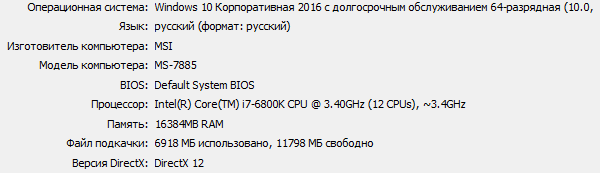
\includegraphics[scale = 1.05]{images/0.png}
	
	\caption{}
	\label{image:1}
\end{figure}

Информация о компиляторе:

\lstinputlisting{listings/0.c.log}

Информация о компоновщике:

\lstinputlisting{listings/0.l.log}

\section{Ход работы}

\subsection{Глава 1. Неименованные каналы}

Посредством pipe-канала можно передавать данные только между двумя процессами. В основе взаимодействия лежит так называемая файловая модель функционирования. Один из процессов создает канал, другой открывает его. После этого оба процесса могут передавать данные через канал в одну или обе стороны, используя для этого функции, предназначенные для работы с файлами, такие как ReadFile и WriteFile.

Анонимные каналы (anonymous channels) Windows обеспечивают однонаправленное (полудуплексное) посимвольное межпроцессное взаимодействие. Каждый канал имеет два дескриптора: дескриптор чтения (read handle) и дескриптор записи (write handle).

После создания канала необходимо передать клиентскому процессу его дескрипторы (или один из них), что обычно делается с помощью механизма наследования. Для наследования описателя нужно, чтобы процесс-потомок создавался функцией CreateProcess с флагом наследования TRUE.

\clearpage

Анонимный канал создается функцией CreatePipe:

\begin{verbatim}
BOOL WINAPI CreatePipe (
    _Out_     PHANDLE                hReadPipe,
    _Out_     PHANDLE                hWritePipe,
    _In_opt_  LPSECURITY_ATTRIBUTES  lpPipeAttributes,
    _In_      DWORD                  nSize
);
\end{verbatim}

\subsubsection{1. Клиент-серверное приложение на основе анонимных каналов}

На сервере создается неименованный канал для связи с процессом-потомком и порождается процесс-потомок. Также на сервере производится запись из консоли в канал. При нажатии на ESC приложение завершается:

\lstinputlisting{listings/p1.1.p.cpp}

Клиент открывает неименованный канал, и считывает из него сообщения. Запись и чтение производится с помощью стандартных потоков stdin и stdout.

\lstinputlisting{listings/p1.1.c.cpp}

Результат передачи от родителя потомку:

\begin{figure}[h!]
	\centering
	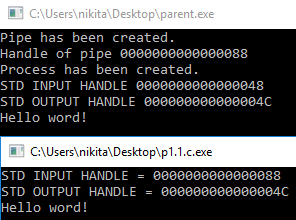
\includegraphics[scale = 1.05]{images/p1_1.png}
	
	\caption{}
	\label{image:2}
\end{figure}

Сообщение было успешно передано.

\subsubsection{2. Эхо-сервер, взаимодействующий с клиентом посредством анонимных каналов}

В программе используется передача дескрипторов через наследование. По причине того, что анонимный канал является полудуплексным, для организации эхо-сервера необходимо создавать 2 канала (для передачи от клиента-серверу и обратно):

\lstinputlisting{listings/p1.2.p.cpp}

Клиентская часть симметрична серверной:

\lstinputlisting{listings/p1.2.c.cpp}

\clearpage

Результат обмена сообщениями:

\begin{figure}[h!]
	\centering
	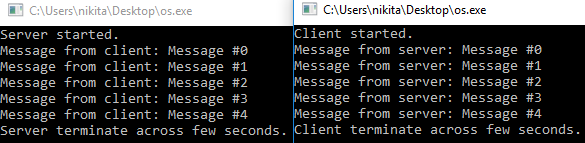
\includegraphics[scale = 1.05]{images/p1_2.png}
	
	\caption{}
	\label{image:3}
\end{figure}

Сообщения были сгенерированы на клиентской стороне, отправлены на сервер. После этого сервер успешно принял сообщения и отослал их назад клиенту.

\subsection{Глава 2. Именованные каналы}

Именованные каналы являются дуплексными, ориентированы на обмен сообщениями и обеспечивают взаимодействие через сеть. Кроме того, один именованный канал может иметь несколько открытых дескрипторов. В сочетании с удобными, ориентированными на выполнение транзакций функциями эти возможности делают именованные каналы пригодными для создания клиент-серверных систем. Обмен данными может быть синхронным и асинхронным.

Для создания именованного канала используется функция CreateNamedPipe. При первом вызове функции CreateNamedPipe происходит создание самого именованного канала, а не просто его экземпляра. Закрытие последнего открытого дескриптора экземпляра именованного канала приводит к уничтожению этого экземпляра (обычно существует по одному дескриптору на каждый экземпляр). Уничтожение последнего экземпляра именованного канала приводит к уничтожению самого канала, в результате чего имя канала становится вновь доступным для повторного использования.

\begin{verbatim}
HANDLE WINAPI CreateNamedPipe(
    _In_      LPCTSTR                lpName,
    _In_      DWORD                  dwOpenMode,
    _In_      DWORD                  dwPipeMode,
    _In_      DWORD                  nMaxInstances,
    _In_      DWORD                  nOutBufferSize,
    _In_      DWORD                  nInBufferSize,
    _In_      DWORD                  nDefaultTimeOut,
    _In_opt_  LPSECURITY_ATTRIBUTES  lpSecurityAttributes
);
\end{verbatim}

После создания именованного канала сервер может ожидать подключения клиента, вызывая функцию ConnectNamedPipe.

\begin{verbatim}
BOOL WINAPI ConnectNamedPipe(
    _In_         HANDLE        hNamedPipe,
    _Inout_opt_  LPOVERLAPPED  lpOverlapped
);
\end{verbatim}

Для подключения клиента к именованному каналу применяется функция CreateFile. С помощью функции WaitNamedPipe процесс может выполнять ожидание момента, когда канал Pipe будет доступен для соединения.

\begin{verbatim}
BOOL WINAPI WaitNamedPipe(
    _In_  LPCTSTR  lpNamedPipeName,
    _In_  DWORD    nTimeOut
);
\end{verbatim}

\subsubsection{1. Программа, обеспечивающая взаимодействие процессов посредством именованных каналов}

Сервер создает именованный канал для двунаправленного использования и ожидает подключения программы-клиента. В цикле сервер получает сообщения от клиента и отправляет их назад:

\lstinputlisting{listings/p2.1.p.cpp}

\clearpage

Клиент на своей стороне открывает канал, пишет в него и читает эхо-ответ. При отправке сообщении "@EXIT@" программа завершается:

\lstinputlisting{listings/p2.1.c.cpp}

\clearpage

Результат клиент-серверного взаимодействия:

\begin{figure}[h!]
	\centering
	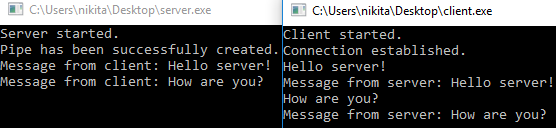
\includegraphics[scale = 1.05]{images/p2_1.png}
	
	\caption{}
	\label{image:4}
\end{figure}

Сообщения отправленные на сервер сразу же возвращаются назад, что соответствует корректной работе эхо-сервера.

\subsubsection{2. Поддержка множества клиентов, блокировка обмена до завершения операций}

Сервер, как и ранее, создает все необходимые ресурсы и переходит в состояние ожидания соединений. Именованный канал создается для чтения и записи. Передача происходит сообщениями, функции передачи и приема блокируются до их окончания:

\lstinputlisting{listings/p2.2.p.cpp}

Клиентский код практически не изменился, за исключением добавления функции WaitNamedPipe:

\lstinputlisting{listings/p2.2.c.cpp}

Результат клиент-серверного взаимодействия с множеством клиентов:

\begin{figure}[h!]
	\centering
	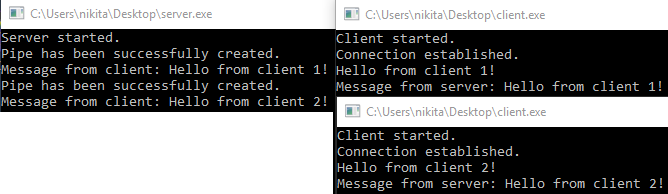
\includegraphics[scale = 0.95]{images/p2_2.png}
	
	\caption{}
	\label{image:5}
\end{figure}

Был запущен сервер и два клиентских окна, после этого каждый клиент послал по сообщению, которые сервер успешно обработал.

\subsubsection{3. Модификация для сетевого обмена информацией}

Для совместной работы компьютеры нужно подсоединить к одной домашней группе. Так же необходимо установить поле DACL защиты объекта в NULL. Параметры защиты именованного канала задаются с помощью структуры SECURITY\_ATTRIBUTES, которая указывается последним параметром в функции CreateNamedPipe.

Модификация сервера для работы по сети:

\lstinputlisting{listings/p2.3.p.cpp}

Модификация клиента для работы по сети:

\lstinputlisting{listings/p2.3.c.cpp}

Сетевые параметры клиента:

\begin{figure}[h!]
	\centering
	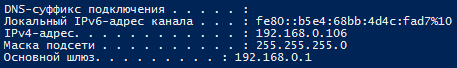
\includegraphics[scale = 0.85]{images/p2_3_client_config.png}
	
	\caption{}
	\label{image:6}
\end{figure}

Сетевые параметры сервера:

\begin{figure}[h!]
	\centering
	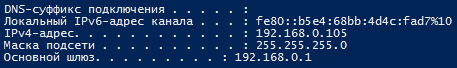
\includegraphics[scale = 0.85]{images/p2_3_server_config.png}
	
	\caption{}
	\label{image:7}
\end{figure}

Отправка клиентского сообщения:

\begin{figure}[h!]
	\centering
	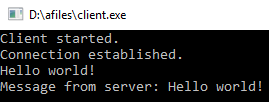
\includegraphics[scale = 0.90]{images/p2_3_client_result.png}
	
	\caption{}
	\label{image:8}
\end{figure}

Прием сообщения удаленным сервером:

\begin{figure}[h!]
	\centering
	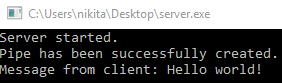
\includegraphics[scale = 0.90]{images/p2_3_server_result.png}
	
	\caption{}
	\label{image:9}
\end{figure}

Компьютеры были объединены в общую домашнюю группу, что позволило им обмениваться сообщениями удаленно при помощи именованных каналов.

\subsection{Глава 3. Сокеты}

WinSock или Windows socket - это интерфейс программного программирования (API) созданный для реализации приложений в сети на основе протокола TCP/IP. Для работы используется WSOCK32.DLL. Windows socket разрабатывался на основе интерфейса Беркли для UNIX, но к ним добавлены функции поддержки событий Windows.

Есть две версии библиотеки WinSock:

\begin{itemize}
	\item \emph{WinSock 1.1} - поддержка только TCP/IP.
	\item \emph{WinSock 2.0} - Поддерка дополнительного программного обеспечения.
\end{itemize}

Спецификация WinSock разделяет функции на три типа:

\begin{itemize}
	\item Функции Беркли.
	\item Информационные функции (получение информации о наименовании доменов, службах, протоколах Internet).
	\item Расширения Windows для функций Беркли.
\end{itemize}

\subsubsection{1 - 3. Многопоточный сервер, обслуживающая множество клиентов, поддерживающий сетевой обмен информацией}

Разработаем программу \emph{TCP} сервера, который в бесконечном цикле ожидает подключения клиентов, создает для каждого из них новый поток, принимает сообщения клиента и отправляет их назад. Также реализована обработка сигнала прерывания для корректного завершения работы всех потоков и закрытия сокетов:

\lstinputlisting{listings/p3.1.p.cpp}

Клиент подключается к серверу, считывает сообщения из консоли и отправляет их серверу, после этого ожидает ответного сообщения сервера. Если было введено пустое сообщение, то клиент завершает работу:

\lstinputlisting{listings/p3.1.c.cpp}

Результат одновременной локальной работы нескольких клиентов:

\begin{figure}[h!]
	\centering
	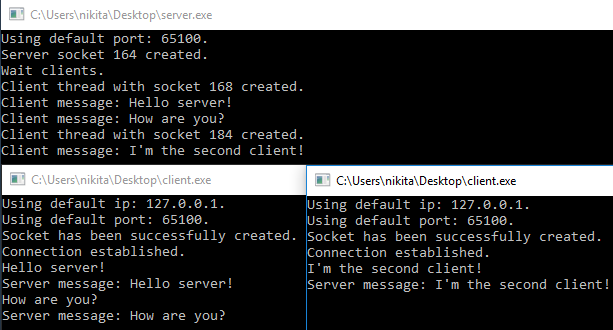
\includegraphics[scale = 0.88]{images/p3_1.png}
	
	\caption{}
	\label{image:10}
\end{figure}

Клиенты успешно установили соединение с сервером, а также осуществили обмен сообщениями.

Однако, в основном сокеты используют для сетевого обмена пакетами. Вышеописанному клиенту и серверу не нужны дополнительные модификации для сетевого обмена. Однако необходимо узнать ip адрес компьютера с сервером и указать его в качестве аргумента командной строки клиента.

Сетевые параметры клиента:

\begin{figure}[h!]
	\centering
	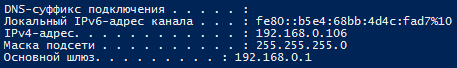
\includegraphics[scale = 0.90]{images/p3_3_client_config.png}
	
	\caption{}
	\label{image:11}
\end{figure}

Сетевые параметры сервера:

\begin{figure}[h!]
	\centering
	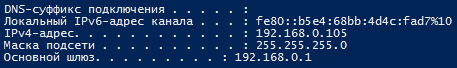
\includegraphics[scale = 0.90]{images/p3_3_server_config.png}
	
	\caption{}
	\label{image:12}
\end{figure}

\clearpage

Отправка клиентского сообщения:

\begin{figure}[h!]
	\centering
	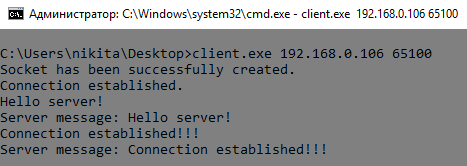
\includegraphics[scale = 0.80]{images/p3_3_client_result.png}
	
	\caption{}
	\label{image:13}
\end{figure}

Прием сообщения удаленным сервером:

\begin{figure}[h!]
	\centering
	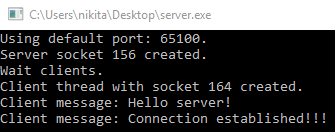
\includegraphics[scale = 0.80]{images/p3_3_server_result.png}
	
	\caption{}
	\label{image:14}
\end{figure}

В первую очередь был получен внутренний ip адрес серверного компьютера. После этого был он был указан в качестве аргумента командной строки для клиента. После этого был осуществлен обмен сообщениями.

\subsubsection{4. Обмен сообщениями между разными операционными системами}

Была реализована сетевая передача сообщений между разными операционными системами. Серверное приложение было запущено на Windows 10 (полные характеристики системы приведены в начале работы), клиентское приложение было запущено на Ubuntu 16.1 (клиентское приложение и система взяты из лабораторной работы "Средства межпроцессорного взаимодействия Linux").

Клиентское приложение для Linux:

\lstinputlisting{listings/p3.4.c.cpp}

Сетевые параметры клиента:

\begin{figure}[h!]
	\centering
	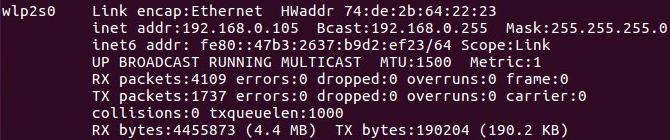
\includegraphics[scale = 0.60]{images/p3_4_client_config.png}
	
	\caption{}
	\label{image:15}
\end{figure}

Результат работы клиента:

\begin{figure}[h!]
	\centering
	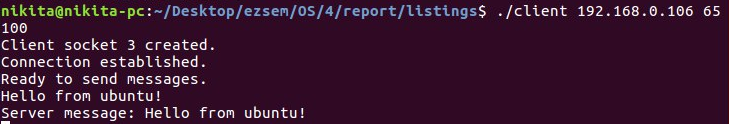
\includegraphics[scale = 0.60]{images/p3_4_client_result.png}
	
	\caption{}
	\label{image:16}
\end{figure}

Результат работы сервера:

\begin{figure}[h!]
	\centering
	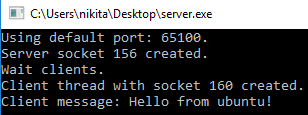
\includegraphics[scale = 0.95]{images/p3_4_server_result.png}
	
	\caption{}
	\label{image:17}
\end{figure}

Сетевой обмен был успешно организован, никаких проблем при реализации не возникло.

\subsubsection{5. Использование портов завершения при большом количестве клиентов}

Порт завершения представляет собой специальный механизм в составе ОС, с помощью которого приложение использует объединение нескольких потоков, предназначенных единственно для цели обработки асинхронных операций ввода/вывода с перекрытием. Для функционирования этой модели необходимо создание специального программного объекта ядра системы, который и был назван "порт завершения". Это осуществляется с помощью функции CreateIoCompletionPort, которая ассоциирует этот объект с одним или несколькими файловыми дескрипторами и который будет управлять перекрывающимися I/O операциями, используя определенное количество потоков для обслуживания завершенных запросов.

\begin{verbatim}
HANDLE WINAPI CreateIoCompletionPort(
    _In_      HANDLE     FileHandle,
    _In_opt_  HANDLE     ExistingCompletionPort,
    _In_      ULONG_PTR  CompletionKey,
    _In_      DWORD      NumberOfConcurrentThreads
);
\end{verbatim}

Реализация сервера, использующего порт завершения:

\lstinputlisting{listings/p3.5.p.cpp}

\clearpage

Для анализа работоспособности на большом количестве клиентов был написан bat скрипт:

\lstinputlisting{listings/p3.5.bat}

Скрипт запускает тысячу клиентов в одном окне.

Производительность тысячи подключенных TCP клиентов до модификации с портами завершения:

\begin{figure}[h!]
	\centering
	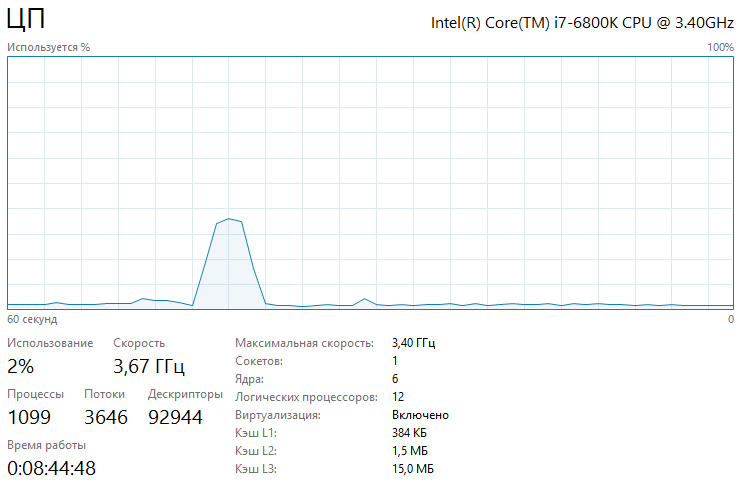
\includegraphics[scale = 0.75]{images/p3_5_old_stat.png}
	
	\caption{}
	\label{image:18}
\end{figure}

Производительность тысячи подключенных TCP клиентов после модификации с портами завершения:

\begin{figure}[h!]
	\centering
	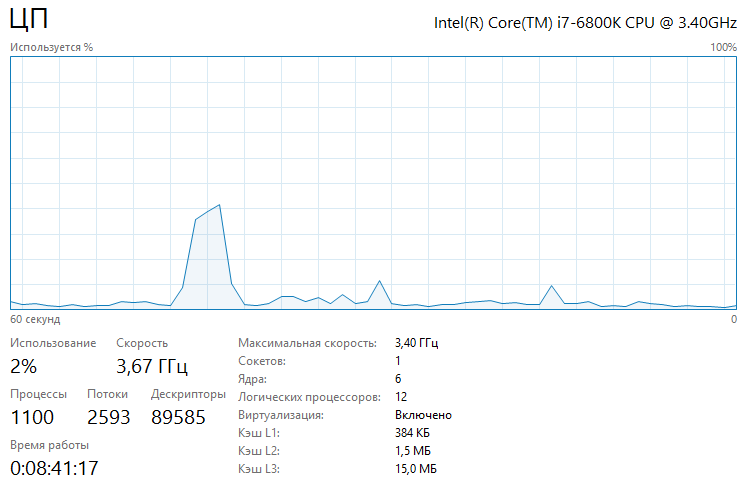
\includegraphics[scale = 0.75]{images/p3_5_new_stat.png}
	
	\caption{}
	\label{image:19}
\end{figure}

Графики практически не отличается, однако есть существенная разница в количестве потоков и дескрипторов. Стоит отметить, что нагрузка в моменты отправки сообщений на порядок ниже при использовании портов завершения.

\subsubsection{6. Оформление приложения в виде службы}

В операционной системе Windows можно запускать приложения в качестве службы. Такое приложение не имеет рабочего терминала и выполняется в фоновом режиме.

Для начала работы службы необходимо дать знать менеджеру служб о том, что мы хотим добавить наше приложение в таблицу служб. Для этого необходимо указать точку входа.

Функция StartServiceCtrlDispatcher связывает службу с SCM (Service Control Manager):

\begin{verbatim}
BOOL WINAPI StartServiceCtrlDispatcher(
    _In_ const  SERVICE_TABLE_ENTRY  *lpServiceTable
);
\end{verbatim}

Функция OpenSCManager позволяет получить экземпляр SCM:

\begin{verbatim}
SC_HANDLE WINAPI OpenSCManager(
    _In_opt_  LPCTSTR  lpMachineName,
    _In_opt_  LPCTSTR  lpDatabaseName,
    _In_      DWORD    dwDesiredAccess
);
\end{verbatim}

Служба создается функцией CreateService:

\begin{verbatim}
SC_HANDLE WINAPI CreateService(
    _In_       SC_HANDLE  hSCManager,
    _In_       LPCTSTR    lpServiceName,
    _In_opt_   LPCTSTR    lpDisplayName,
    _In_       DWORD      dwDesiredAccess,
    _In_       DWORD      dwServiceType,
    _In_       DWORD      dwStartType,
    _In_       DWORD      dwErrorControl,
    _In_opt_   LPCTSTR    lpBinaryPathName,
    _In_opt_   LPCTSTR    lpLoadOrderGroup,
    _Out_opt_  LPDWORD    lpdwTagId,
    _In_opt_   LPCTSTR    lpDependencies,
    _In_opt_   LPCTSTR    lpServiceStartName,
    _In_opt_   LPCTSTR    lpPassword
);
\end{verbatim}

Функция OpenService в зависимости от параметров запускает или останавливает службу:

\begin{verbatim}
SC_HANDLE WINAPI OpenService(
    _In_  SC_HANDLE  hSCManager,
    _In_  LPCTSTR    lpServiceName,
    _In_  DWORD      dwDesiredAccess
);
\end{verbatim}

Сервер был модифицирован следующим образом: в зависимости от аргумента командной строки install, start, remove устанавливается, запускается и удаляется служба соответственно:

\lstinputlisting{listings/p3.6.p.cpp}

\clearpage

Установка, запуск и удаление службы:

\begin{figure}[h!]
	\centering
	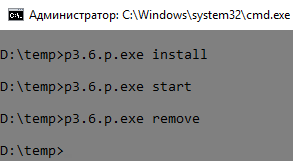
\includegraphics[scale = 0.8]{images/p3_6_api.png}
	
	\caption{}
	\label{image:20}
\end{figure}

Созданная служба после установки:

\begin{figure}[h!]
	\centering
	
\includegraphics[scale = 1.0]{images/p3_6_service.png}
	
	\caption{}
	\label{image:21}
\end{figure}

Процесс привязанный к службе:

\begin{figure}[h!]
	\centering
	
\includegraphics[scale = 0.9]{images/p3_6_process.png}
	
	\caption{}
	\label{image:22}
\end{figure}

Стоит отметить, что СИСТЕМА является владельцем этого процесса.

\subsubsection{7. Реализация обмена на основе UDP}

Разработаем программу \emph{UDP} сервера. В отличии от \emph{TCP}, соединение не устанавливается, поэтому отсутствуют функции \emph{listen} и \emph{accept}. Также не имеет большого смысла регистрировать отдельный поток для каждого клиента. Сервер в бесконечном цикле принимает сообщения от клиента и отправляет их назад:

\lstinputlisting{listings/p3.7.p.cpp}

Клиент подключается к серверу, считывает сообщения из консоли и отправляет их серверу, после этого ожидает ответного сообщения сервера. В отличие от \emph{TCP} отсутствует функция \emph{connect}, отвечающая за установление соединения. Если было введено пустое сообщение, то клиент завершает работу:

\lstinputlisting{listings/p3.7.c.cpp}

\clearpage

Протестируем клиент-серверное приложение:

\begin{figure}[h!]
	\centering
	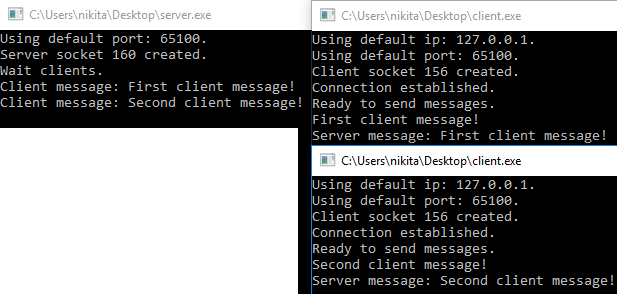
\includegraphics[scale = 0.9]{images/p3_7.png}
	
	\caption{}
	\label{image:23}
\end{figure}

В первую очередь был запущен сервер два клиента. Клиенты отправляют сообщения серверу, после чего сервер завершает свою работу. В связи с тем что отсутствует установление соединения \emph{UDP}, клиенты не узнают о том, что сервер отключился. Для обхода такой ситуации обычно с какой то очередностью серверу отправляется пакет, если от сервера пакет не пришел - значит сервер недоступен.

\subsection{Глава 4. Сигналы в Windows}

Данное средство IPC в Windows не поддерживается в том смысле, в котором оно используется в Unix-системах. Однако, например, консольному приложению можно посылать сигналы CTRL+C и CTRL+BREAK. Система может посылать приложению сигналы: CTRL\_CLOSE\_EVENT, CTRL\_LOGOFF\_EVENT и CTRL\_SHUTDOWN\_EVENT, когда пользователь закрывает консоль, выходит из системы или когда система завершает работу. По получению данных сигналов процесс может произвести корректное завершение.

С помощью функции SetConsoleCtrlHandler можно установить обработчик на эти сигналы, но отправить сигнал другому приложению невозможно.

\begin{verbatim}
BOOL WINAPI SetConsoleCtrlHandler(
    _In_opt_  PHANDLER_ROUTINE  HandlerRoutine,
    _In_      BOOL              Add
);
\end{verbatim}

Обработчики сигналов объединены в список. Когда приходит сигнал, вызывается последний зарегистрированный обработчик (при этом запускается отдельный поток). Если этот обработчик возвращает FALSE (он не обрабатывает этот сигнал), то вызывается следующий. Если все обработчики вернули FALSE, вызовется обработчик по умолчанию, который по умолчанию завершает процесс.

\subsubsection{1. Создание обработчика сигналов завершения для консольного приложения}

Была написана программа, которая устанавливает обработчик сигнала функцией SetConsoleCtrlHandler и выводит название завершающего сигнала. Также в зависимости от сигнала производится звуковой сигнал определенной частоты: 

\lstinputlisting{listings/p4.1.cpp}

Результат работы программы:

\begin{figure}[h!]
	\centering
	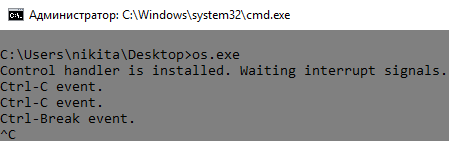
\includegraphics[scale = 0.9]{images/p4_1.png}
	
	\caption{}
	\label{image:24}
\end{figure}

Реализуем собственный обработчик прерывания. При завершении приложения комбинацией клавиш Ctrl+C реализована проверка случайного нажатия. Если пользователь нажал комбинацию случайно, то приложение продолжает работу, а если нет то запрашивается еще одно нажатие:

\lstinputlisting{listings/p4.1.i.cpp}

\subsection{Глава 5. Разделяемая память}

Потоки одного процесса могут разделять общую память этого процесса. У каждого процесса – свое изолированное адресное пространство. Кроме рассмотренных выше средств передачи информации между процессами или потоками разных процессов, одно из наиболее эффективных – использование общей памяти, доступ к которой обеспечивается со стороны каждого процесса. ОС Windows поддерживает такое средство, как именованная, совместно используемая память. 

Первый участвующий в обмене информацией процесс создает объект проекции файла при помощи вызова функции CreateFileMapping. Используя флажок PAGE\_READWRITE, задается доступ по чтению и записи в память через представление данных файла в адресном пространстве процесса.

\begin{verbatim}
HANDLE WINAPI CreateFileMapping(
    _In_      HANDLE                 hFile,
    _In_opt_  LPSECURITY_ATTRIBUTES  lpAttributes,
    _In_      DWORD                  flProtect,
    _In_      DWORD                  dwMaximumSizeHigh,
    _In_      DWORD                  dwMaximumSizeLow,
    _In_opt_  LPCTSTR                lpName
);
\end{verbatim}

Процесс затем использует дескриптор объекта возвращаемый функцией CreateFileMapping, при вызове функции MapViewOfFile. Эта функция создает представление файла в адресном пространстве процесса и возвращает указатель на представление данных файла для их дальнейшего использования.

\begin{verbatim}
LPVOID WINAPI MapViewOfFile(
    _In_  HANDLE  hFileMappingObject,
    _In_  DWORD   dwDesiredAccess,
    _In_  DWORD   dwFileOffsetHigh,
    _In_  DWORD   dwFileOffsetLow,
    _In_  SIZE_T  dwNumberOfBytesToMap
);
\end{verbatim}

Другой процесс может получить доступ к тем же данным при помощи вызова функции OpenFileMapping с тем же самым именем, что и первый процесс, а затем использовать функцию MapViewOfFile, чтобы получить свой указатель на представление данных файла.

\begin{verbatim}
HANDLE WINAPI OpenFileMapping(
    _In_  DWORD    dwDesiredAccess,
    _In_  BOOL     bInheritHandle,
    _In_  LPCTSTR  lpName
);
\end{verbatim}

\subsubsection{1. Взаимодействие двух процессов через совместно используемую именованную память}

Процесс-читатель считывает определенное количество сообщений (ITERATIONS\_COUNT) от процесса-писателя, после чего завершает свою работу:

\lstinputlisting{listings/p5.r.cpp}

Процесс-писатель бесконечно генерирует случайные числа и записывает их в разделяемую память:

\lstinputlisting{listings/p5.w.cpp}

Результат совместной работы процесса-писателя и процесса-читателя:

\begin{figure}[h!]
	\centering
	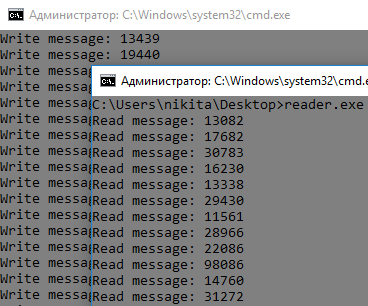
\includegraphics[scale = 0.9]{images/p5.png}
	
	\caption{}
	\label{image:25}
\end{figure}

Процесс-писатель успешно сгенерировал набор случайных чисел, а процесс-читатель успешно считал их из разделяемой памяти.

\subsection{Глава 6. Почтовые слоты}

Для решения задачи передачи данных посредством почтовых слотов необходимо воспользоваться функциями CreateMailslot и CreateFile. 

\begin{verbatim}
HANDLE WINAPI CreateMailslot(
    _In_      LPCTSTR                lpName,
    _In_      DWORD                  nMaxMessageSize,
    _In_      DWORD                  lReadTimeout,
    _In_opt_  LPSECURITY_ATTRIBUTES  lpSecurityAttributes
);
\end{verbatim}

Сервер создает почтовый слот и считывает оттуда данные при помощи функции ReadFile. Клиент использует функцию CreateFile с именем почтового слота в качестве имени файла. Таким образом, клиент присоединяется к уже существующему почтовому слоту, созданному сервером. Запись данных в почтовый слот происходит при помощи функции WriteFile.

\subsubsection{1. Обмен сообщениями посредством почтовых слотов на одном компьютере}

Сервер считывает клиентские сообщения посредством почтовых слотов:

\lstinputlisting{listings/p6.1.p.cpp}

Клиентская программа считывает сообщения с консоли и отправляет их на сервер:

\lstinputlisting{listings/p6.1.c.cpp}

Результат передачи сообщения в пределах одного компьютера:

\begin{figure}[h!]
	\centering
	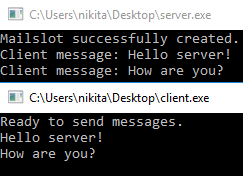
\includegraphics[scale = 0.9]{images/p6_1.png}
	
	\caption{}
	\label{image:26}
\end{figure}

\subsubsection{1. Обмен сообщениями посредством почтовых слотов в локальной сети}

Для выполнения удаленного доступа, то есть использования почтовых слотов для передачи данных по сети, необходимо указать вместо точки в имени почтового слота адрес компьютера в сети:

\begin{verbatim}
static const char* MAILSLOT_NAME = "\\\\DESKTOP-MK2E3MO\\mailslot\\MyMailSlot";
\end{verbatim}

После этого запускаем сервер и клиент на разных компьютерах. Результат приема сообщения сервером:

\begin{figure}[h!]
	\centering
	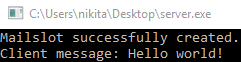
\includegraphics[scale = 1.2]{images/p6_2_result.png}
	
	\caption{}
	\label{image:27}
\end{figure}

Рассмотрим пришедший пакет программой WireShark:

\begin{figure}[h!]
	\centering
	
\includegraphics[scale = 0.9]{images/p6_2_wireshark_ip.png}
	
	\caption{}
	\label{image:28}
\end{figure}

\clearpage

Содержимое пришедшего пакета:

\begin{figure}[h!]
	\centering
	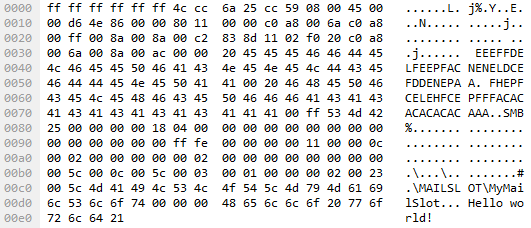
\includegraphics[scale = 0.85]{images/p6_2_wireshark_package.png}
	
	\caption{}
	\label{image:29}
\end{figure}

Как видно из записей трафика на машину сервер (192.168.0.106) пришли данные от клиента (192.168.0.105) по протоколу SMB Mailslot. Если подробно рассмотреть сами передаваемые данные, то в конце можно заметить текст, который успешно был передан.

\subsubsection{2. Широковещательная передача данных посредством почтовых слотов}

При создании почтовых слотов с одинаковым именем на нескольких компьютерах домена возможна широковещательная рассылка сообщений клиентов. Один клиентский процесс может посылать сообщения сразу всем этим серверным процессам. Для этого заменим в клиенте имя компьютера на символ "*":

\begin{verbatim}
static const char* MAILSLOT_NAME = "\\\\*\\mailslot\\MyMailSlot";
\end{verbatim}

Запустим на каждой из машин по серверу и отправим широковещательный пакет. Результат приема сообщения серверами:

\begin{figure}[h!]
	\centering
	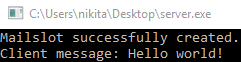
\includegraphics[scale = 1.1]{images/p6_3_result.png}
	
	\caption{}
	\label{image:30}
\end{figure}

Рассмотрим пришедший пакет программой WireShark:

\begin{figure}[h!]
	\centering
	
\includegraphics[scale = 0.85]{images/p6_3_wireshark_ip.png}
	
	\caption{}
	\label{image:31}
\end{figure}

Содержимое пришедшего пакета:

\begin{figure}[h!]
	\centering
	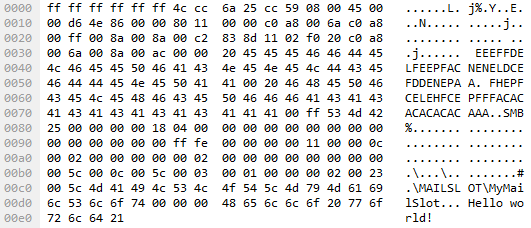
\includegraphics[scale = 0.85]{images/p6_3_wireshark_package.png}
	
	\caption{}
	\label{image:32}
\end{figure}

Как и требовалось ожидать, широковещательные сообщения были успешно отправлены клиентами и приняты серверами.

\section{Вывод}

В ходе данной работы были рассмотрены следующие средства межпроцессного взаимодействия в операционных системах семейства Windows: именованные и неименованные каналы, сокеты, разделяемая память, почтовые слоты.

\begin{itemize}
	\item Неименованные каналы Windows обеспечивают однонаправленное посимвольное межпроцессное взаимодействие. Каждый канал имеет два дескриптора: дескриптор чтения и дескриптор записи. Дескрипторы каналов часто бывают наследуемыми. Чтобы канал можно было использовать для IPC, должен существовать еще один процесс, и для этого процесса требуется один из дескрипторов канала. Анонимные каналы обеспечивают только однонаправленное взаимодействие, для двухстороннего взаимодействия необходимы два канала.
	
	\item Именованные каналы обеспечивают межпроцессное взаимодействие между сервером и одним или несколькими клиентами. Они предоставляют больше функциональных возможностей, чем анонимные каналы, которые обеспечивают межпроцессное взаимодействие на локальном компьютере. Именованные каналы поддерживают дуплексную связь по сети, несколько экземпляров сервера, взаимодействие, основанное на сообщениях и олицетворение клиента, что позволяет подключаемым процессам использовать собственные наборы разрешений на удаленных серверах. Использовать именованные каналы для связи по сети возможно только для компьютеров с ОС Windows, подключенных к одной домашней группе.
	
	\item Возможность взаимодействия с другими системами обеспечивается в Windows поддержкой сокетов. Сокет – это оконечная точка соединения, которая идентифицируется четырьмя4 значениями: IP адрес отправителя, порт отправителя, IP адрес получателя, порт получателя.
	
	\item Механизм сигналов как IPC отсутствует в ОС Windows. Процессы не могут отправлять сигналы другим процессам для обмена информацией. Присутствует 2 сигнала которые пользователь может отправлять приложению с клавиатуры: Ctrl+C и Ctrl+Break. Так же система может посылать приложению сигналы, когда пользователь закрывает консоль, выходит из системы или, когда система завершается.
	
	\item ОС Windows поддерживает такое средство, как именованная, совместно используемая память. Разделяемая память позволяет обмениваться информацией между двумя процессами.
	
	\item Почтовый слот – механизм синхронизации, иначе называемый почтовый ящик. Каждый слот реализуется как псевдофайл в оперативной памяти и содержит некоторое количество записей, которые могут быть прочтены всеми компьютерами в сетевом домене. Используя почтовые слоты можно передавать данные между компьютерами в локальной сети. При создании почтовых слотов с одинаковым именем на нескольких компьютерах домена возможна широковещательная рассылка сообщений клиентов. Один клиентский процесс может посылать сообщения сразу всем этим серверным процессам посредством широковещательных запросов.
\end{itemize}



\section{Список литературы}

\begin{itemize}
	\item CreatePipe function [Электронный ресурс]. — URL: \href{https://msdn.microsoft.com/ru-ru/library/windows/desktop/aa365152(v=vs.85).aspx}{https://msdn.microsoft.com/ru-ru/library/windows/\linebreak desktop/aa365152(v=vs.85).aspx} (дата обращения 11.01.2017).
	
	\item CreateNamedPipe function [Электронный ресурс]. — URL: \href{https://msdn.microsoft.com/ru-ru/library/windows/desktop/aa365150(v=vs.85).aspx}{https://msdn.microsoft.com/ru-ru/library/windows/\linebreak desktop/aa365150(v=vs.85).aspx} (дата обращения 11.01.2017).
	
	\item Что такое Windows Sockets [Электронный ресурс]. — URL: \href{http://www.firststeps.ru/mfc/net/socket/r.php?1}{http://www.firststeps.ru/mfc/net/socket/r.php?1} (дата обращения 11.01.2017).
	
	\item CreateService function [Электронный ресурс]. — URL: \href{https://msdn.microsoft.com/ru-ru/library/windows/desktop/ms682450(v=vs.85).aspx}{https://msdn.microsoft.com/ru-ru/library/windows/\linebreak desktop/ms682450(v=vs.85).aspx} (дата обращения 11.01.2017).
	
	\item SetConsoleCtrlHandler function [Электронный ресурс]. — URL: \href{https://msdn.microsoft.com/ru-ru/library/windows/desktop/ms686016(v=vs.85).aspx}{https://msdn.microsoft.com/ru-ru/library/windows/\linebreak desktop/ms686016(v=vs.85).aspx} (дата обращения 11.01.2017).
	
	\item CreateFileMapping function [Электронный ресурс]. — URL: \href{https://msdn.microsoft.com/ru-ru/library/windows/desktop/aa366537(v=vs.85).aspx}{https://msdn.microsoft.com/ru-ru/library/windows/\linebreak desktop/aa366537(v=vs.85).aspx} (дата обращения 11.01.2017).
	
	\item CreateMailslot function [Электронный ресурс]. — URL: \href{https://msdn.microsoft.com/ru-ru/library/windows/desktop/aa365147(v=vs.85).aspx}{https://msdn.microsoft.com/ru-ru/library/windows/\linebreak desktop/aa365147(v=vs.85).aspx} (дата обращения 11.01.2017).	
\end{itemize}

\end{document}